\section{Overview}

GEMC \cite{gemc} is a c++ framework that uses Geant4 \cite{geant4} to simulate the passage of particles through matter. It provides:
\begin{itemize}
	\item application independent geometry description
	\item easy interface to build / run experiments
	\item cad/gdml imports
\end{itemize}

The simulation parameters are stored in external databases and are used to define the Geant4 objects at run time. This includes:
\begin{itemize}
	\item geometry
	\item materials
	\item mirrors
	\item physics list
	\item database constants
	\item digitization
	\item electromagnetic fields
\end{itemize}

Particles are transported through matters and produce radiation, hits, secondaries.
gemc then collects the Geant4 results and produce the output specified by the user.
The design of the framework is summarized in \F{gemcDesign}

\begin{figure}
	\centering
	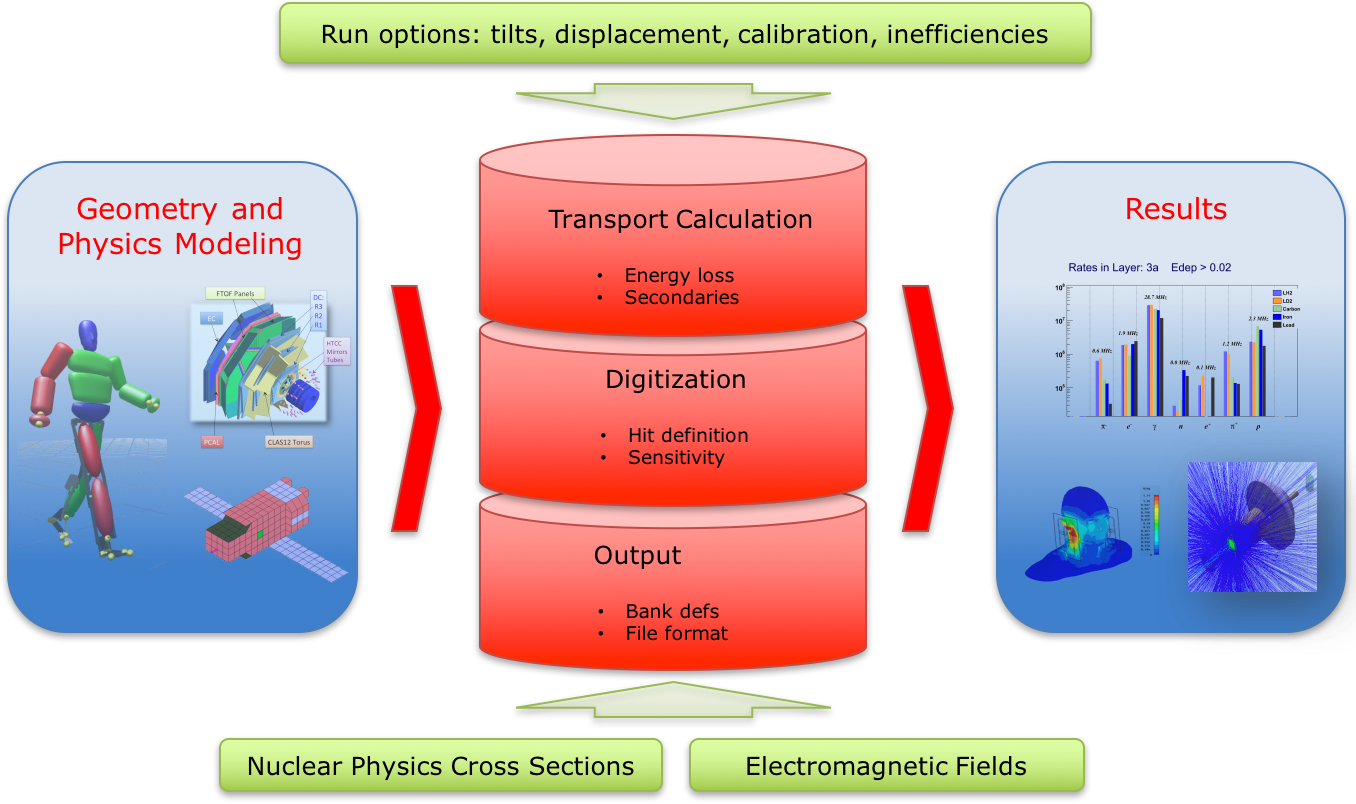
\includegraphics[width=0.98\columnwidth,keepaspectratio]{img/gemcDesign.png}
	\caption{The architecture of GEMC. The Geant4 objects are defined in external database. Geant4 is used to simulate the
             passage of particles through materials, and hits are digitized with plugins defined by users
             and collected in user-defined outputs. }
	\label{fig:gemcDesign}
\end{figure}


\subsection{Geometry and Materials Import}

The geometry and material are stored external databases that can be mysql tables or text files that mimic the mysql tables.
The databases can be defined using the following factories:

\begin{itemize}
	\item GEMC native API (perl or python)
	\item geometry service
	\item cad (stl, ply, obj formats)
	\item gdml, c++ plugins (not used in CLAS12)
\end{itemize}

The GEMC native API repository is \url{https://github.com/gemc/api}. The geometry service code repository is
\url{https://github.com/JeffersonLab/clas12-offline-software/blob/development/common-tools/clas-jcsg/src/main/java/org/jlab/detector/geant4/v2/}


\subsubsection{Geometry database using native API or geometry service}

An example of the code to define and store a Geant4 volume in external databases is shown below. The
numbers are typically hardcoded, come from a calibration databases or are defined in the geometry service. The material
has a similar interface.

\begin{lstlisting}[language=Perl]
my %detector = init_det();

$detector{"name"}        = "shield";
$detector{"mother"}      = "root";
$detector{"description"} = "bst";
$detector{"color"}       = "88aaff";
$detector{"pos"}         =  "0*cm 1*cm 2*cm" ;
$detector{"material"}    = "G4_W";
$detector{"type"}        = "Tube";
$detector{"dimensions"}  = "0*mm 10*mm 20*mm 0*deg 260*deg";
$detector{"visible"}     = 1;
$detector{"style"}       = 1;
print_det(\%configuration, \%detector);

\end{lstlisting}


\subsubsection{Importing CAD volumes from the engineering model}

The Hall-B detectors and their supports are designed with 3D CAD software. This includes a reference system and the
hierarchy of all detector elements, down to details like nuts and bolts.

The CAD models are exported into STP files \cite{stepFiles}.
In order to import them into a Geant4 simulation, first the volumes relevant to the simulation are selected, see \F{cadSelection}.

\begin{figure}
	\centering
	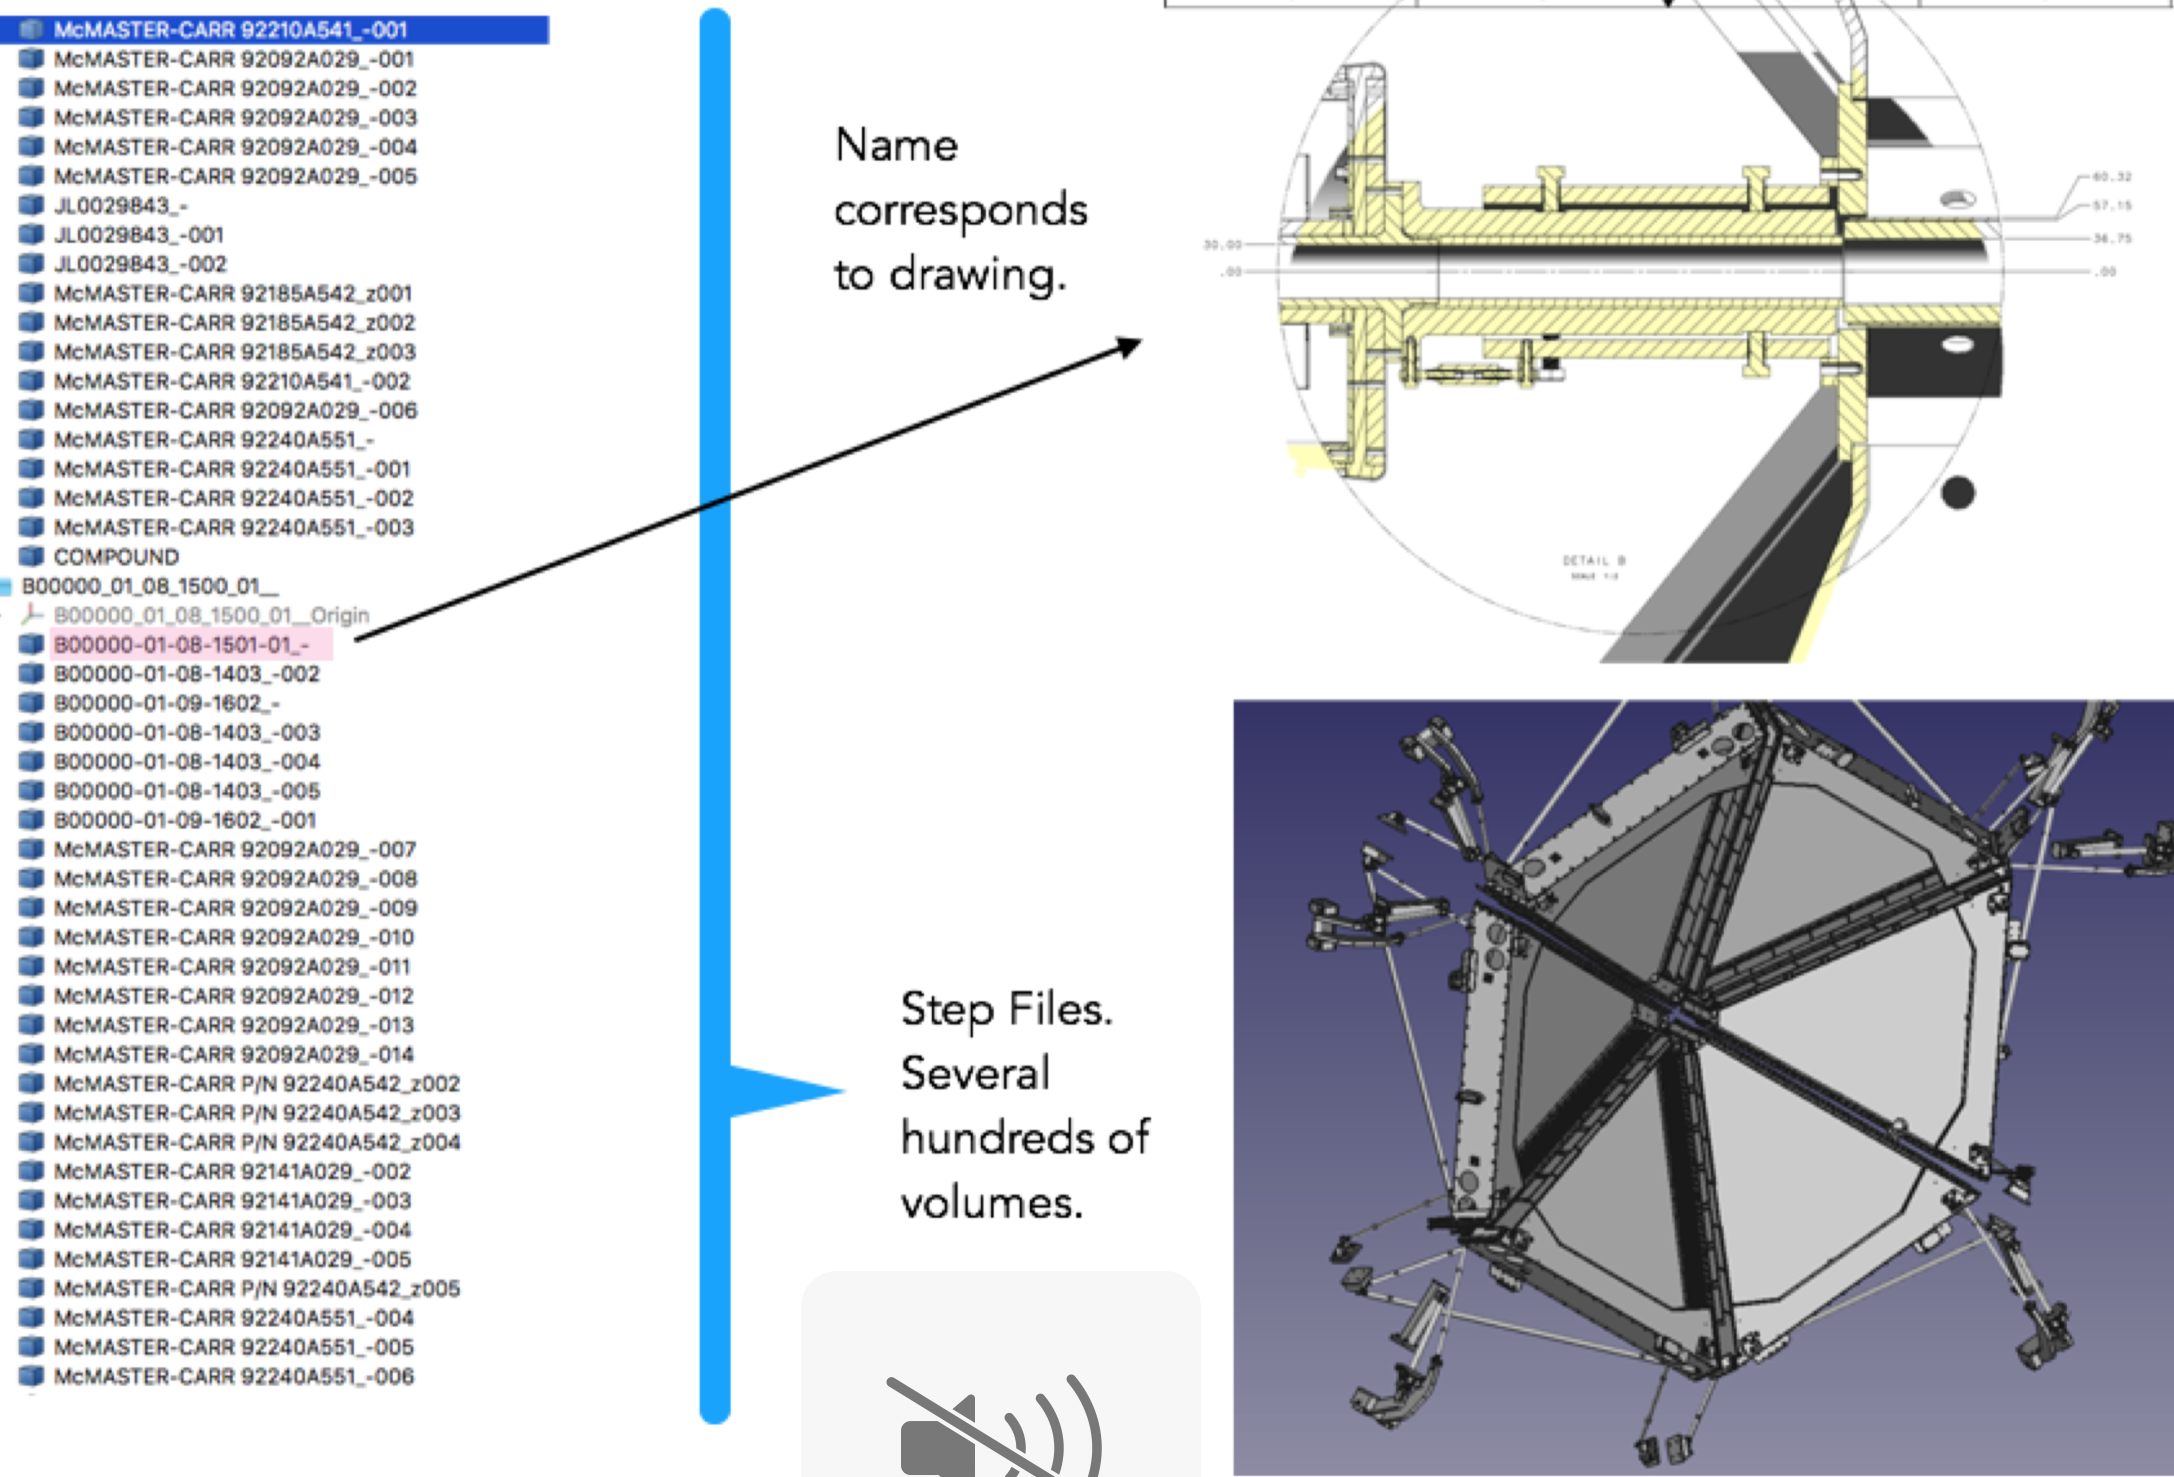
\includegraphics[width=0.98\columnwidth,keepaspectratio]{img/cadSelection.png}
	\caption{The selection of the volumes that will be used in the GEMC Geant4 simulation.
             This typically involves filtering out unnecessary volumes that are not in the active region.}
	\label{fig:cadSelection}
\end{figure}

The elements in the STP file are then ``tessellated'': several polygon shapes are created to define a Geant4 volume.
The software used to do this is FreeCad \cite{freeCad}. An example of tessellation showing the polygon shapes
is shown in \F{targetScatteringChamber}.

The simulated CAD import is as close to reality as the engineering model is close to reality.
We did encounter differences between the STP files, the drawings and reality in a few occasions and worked
out a workflow to eliminate any discrepancy, see \F{cadValidation}.


\begin{figure}
	\centering
	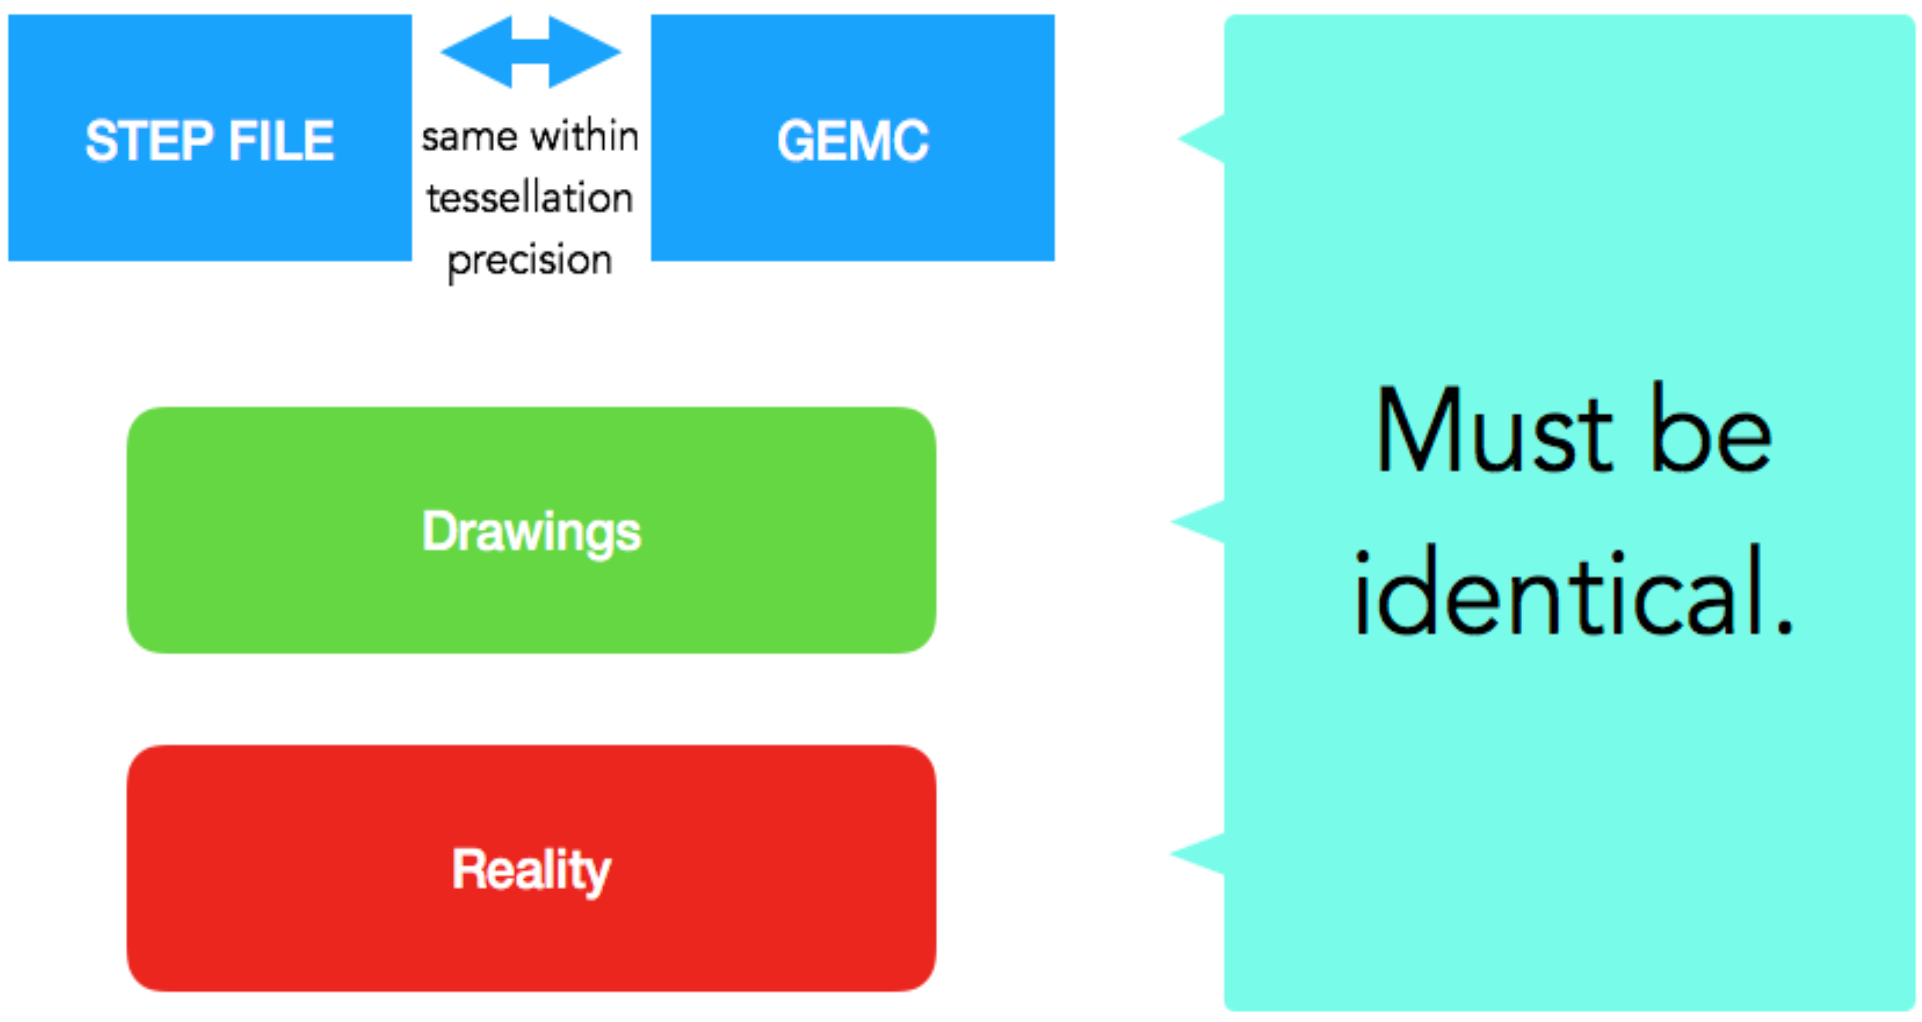
\includegraphics[width=0.95\columnwidth,keepaspectratio]{img/cadValidation.png}
	\caption{There are four possible representation of a volume: the one coming from the STP file
             and the tessellated one are exactly the same object (within the tessellation precision).
             In some cases, certain elements and their sizes and positions did not match the drawings.
             In other cases, they did not match what was built and measured, or their position did not
             match the survey. To eliminate these occurrences physicists and engineers worked until
             the final iteration of a volume was the same in all 4 models: STP/GEMC, Drawings and Reality}
	\label{fig:cadValidation}
\end{figure}

An example of the cad validation is shown in \F{cadValidationExample}.

\begin{figure}
	\centering
	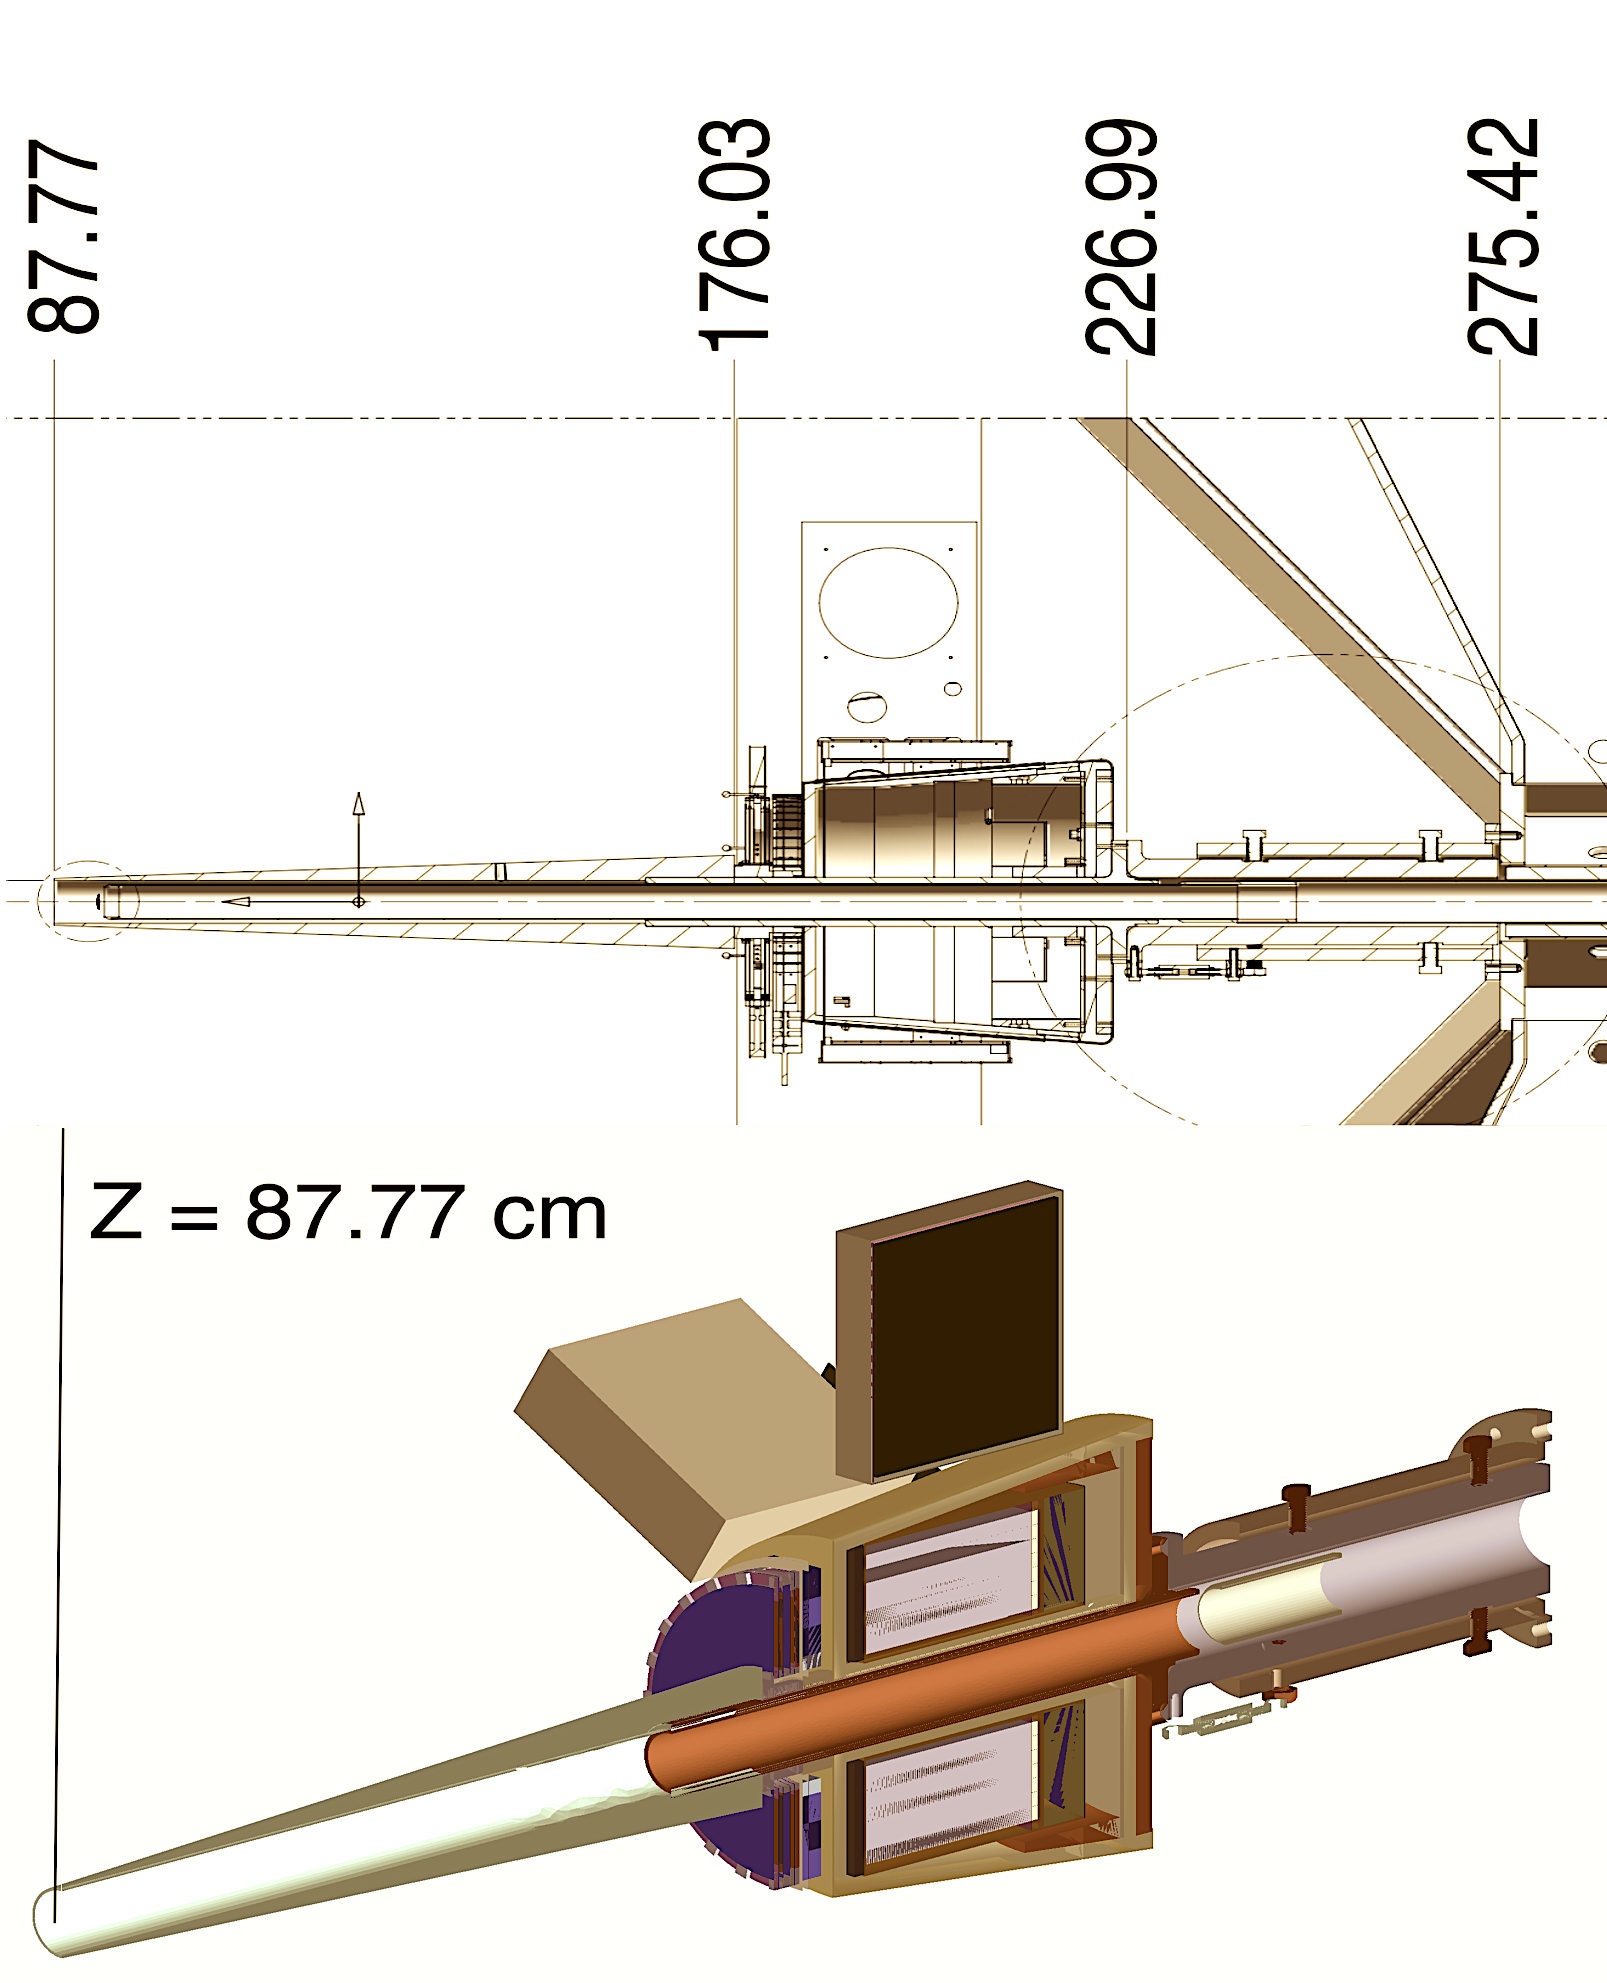
\includegraphics[width=0.95\columnwidth,keepaspectratio]{img/cadValidationExample.png}
	\caption{An example of comparing the GEMC simulation to the drawings. Top: engineering drawings of
             the CLAS12 beamline and shielding. The start of the Moeller shielding is 87.77 cm downstream
             of the target center. Bottom: a geantino is shot vertically at z=87.77 cm, showing that the
             Geant4 cone position agrees with the drawings.}
	\label{fig:cadValidationExample}
\end{figure}



\subsection{Magnetic Fields}
The magnetic fields are loaded from ascii files. The following Geant4 parameters are loaded from
command line options or configuration files at run time:

\begin{itemize}
	\item minStep: minimum step in the magnetic field
	\item integralAlgorithm: compute the field value from the closest cell or using a linear interpolation
	\item interpolationMethod: interpolation algorithm, such as G4ClassicalRK4, G4SimpleRunge, etc
\end{itemize}

The implementation of the CLAS12 magnetic fields is described in \ref{clas12FieldMaps}.

\subsection{Event Time Window and Hit definition}
The Geant4 sensitive volumes are associated with a GEMC identifier that contains hierarchical information such as mother volumes
and volume copy number.

Each detector is associated with a time quantity to mimic the readout electronic time window.

The time window and identifier define a GEMC hit from a series of Geant4 steps: all the steps in a given identifier that are within the time window
are part of the same GEMC hit. The algorithm is illustrated in \F{hitDefinition}.

\begin{figure}
	\centering
	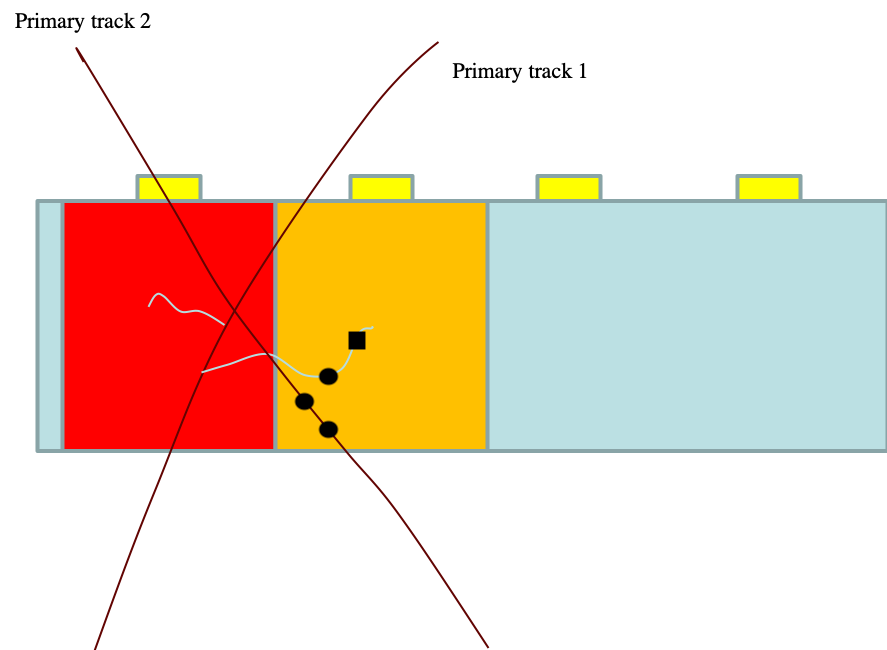
\includegraphics[width=0.95\columnwidth,keepaspectratio]{img/hitDefinition.png}
	\caption{The GEMC Hit definition algorithm. Two sensitive cells, in red and yellow, are hit by four particles, two primaries and two secondaries.
             The Geant4 steps in the yellow sensitive cell are drawn explicitly. The circle steps generated by both the primary track $\#2$ and the secondary
             from track $\#1$ are within the time window and therefore are all part of the same GEMC hit. The single square step generated by the secondary
             from track $\#1$ comes after and does not fall in the circle time window, therefore it is part of a new GEMC hit.}
	\label{fig:hitDefinition}
\end{figure}

\subsection{Process ID}

A "processID" method can be implemented by some digitization algorithm to modify or add GEMC identifiers to each Geant4 step. For CLAS12 this happens in two
cases, detailed for each detector:

\begin{itemize}
	\item a paddle is hit but two outputs are produced because there is one PMT at each end of the scintillator. This
          is the case for CTOF, CND, FTOF.
    \item some hardware elements are not present in the simulation. This is the case for Drift Chambers, where the volumes do not contain
          the individual wires. In this case the wire id is calculated based on the position of the hit in the mother volume. In CLAS12 this mechanism
          is adopted by the DC, BST and Micromegas.
\end{itemize}


\subsection{Detectors and Hit Process Plugin Mechanism}
The detector are associated with c++ digitization routines at run time, see \F{pluginsAssociation}

\begin{figure}
	\centering
	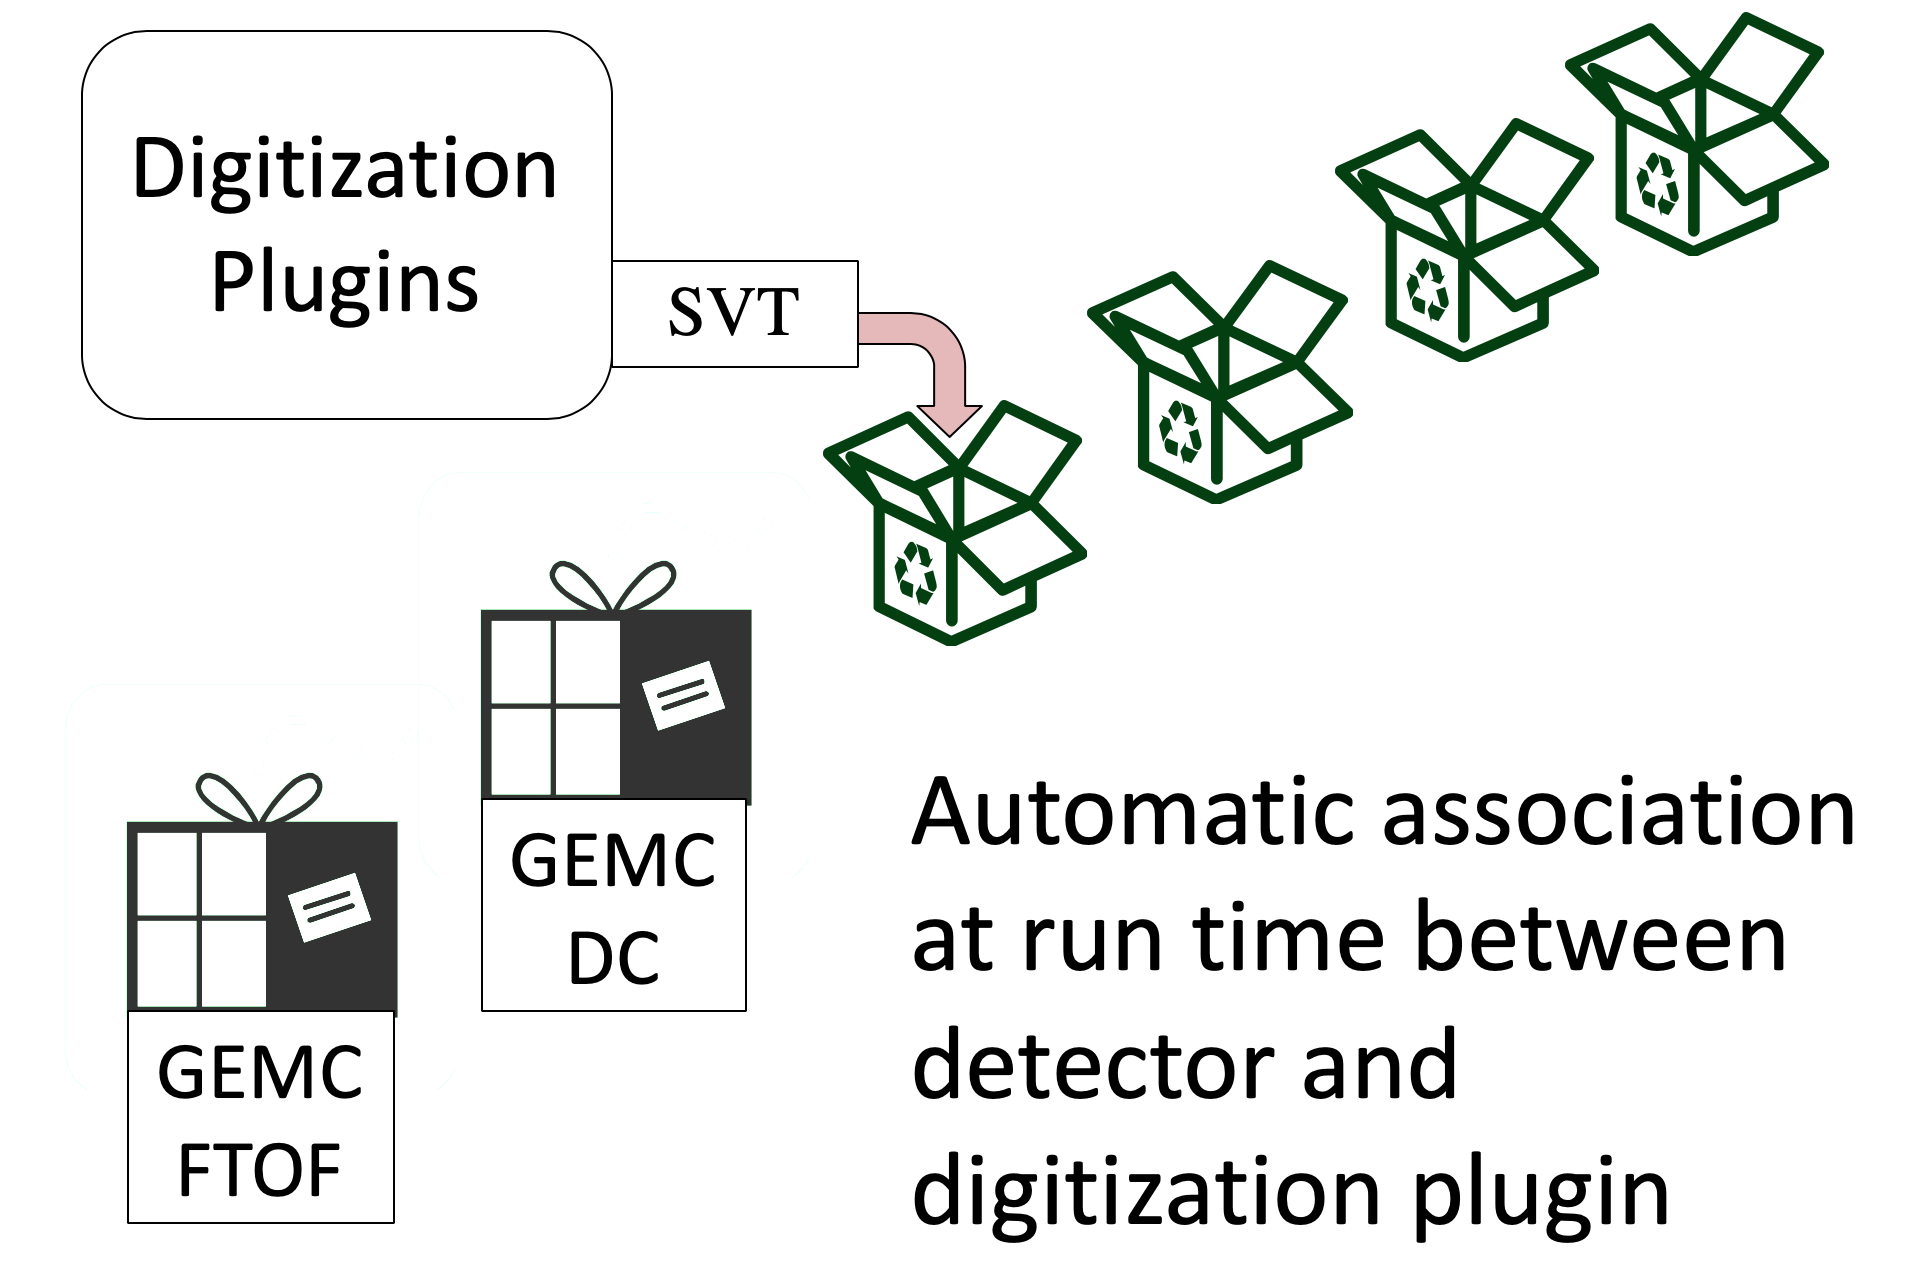
\includegraphics[width=0.95\columnwidth,keepaspectratio]{img/pluginsAssociation.png}
	\caption{Hit Process Digitization Plugin association. The detector are associated by name with the hit process routine plugins at run time:
			 The routine are registered in the hit process map and are called during digitization.}
	\label{fig:pluginsAssociation}
\end{figure}

This allows the routines to
be developed independently from the core code. Abstract methods can be derived in the individual detectors hit processes
to define the treatment of the Geant4 steps within the detector time window to provide three kind of outputs:

\begin{itemize}
	\item a bank with digitized variables for each hit
	\item a bank with digitized variables for Geant4 step
	\item a bank with an analog voltage versus time signal for each Geant4 hit
\end{itemize}

The digitized banks are detailed in each detector subsystem, for example in \ref{tab:bstBank}.

\subsection{True Information}

The true information is saved in the output when requested, per detector. The true information can
be integrated (one variable entry per GEMC hit) or verbose (one variable entry per Geant4 step).
The true information variables are summarized in Table \ref{tab:trueInformation}.

\begin{table}[h]
	\small
	\begin{center}
		\begin{tabular}{| c | c |}
			\hline \hline
			Variable    & Description  \\
			\hline
				pid         &   ID of the FP                     \\
				mpid        &   ID of the mother of the FP \\
				tid         &   Track ID of the FP\\
				mtid        &   Track ID of the mother of the FP  \\
				otid        &   Track ID of the ancestor of the FP \\
				trackE      &   Total energy of the FP \\
				totEdep     &   Total energy deposited (in MeV) \\
				avg\_x      &   Average X position  (in mm) \\
				avg\_y      &   Average Y position  \\
				avg\_z      &   Average Z position  \\
				avg\_lx     &   Average local X position \\
				avg\_ly     &   Average local Y position \\
				avg\_lz     &   Average local Z position \\
				px          &   x  of momentum of the FP (in MeV) \\
				py          &   y  of momentum of the FP \\
				pz          &   z  of momentum of the FP \\
				vx          &   x  of the FP's origin (in mm) \\
				vy          &   y  of the FP's origin \\
				vz          &   z  of the FP's origin \\
				mvx         &   x  of the FP mother's origin\\
				mvy         &   y  of the FP mother's origin \\
				mvz         &   z  of the FP mother's origin \\
				avg\_t      &   Average time \\
				nsteps      &   Number of Geant4 steps \\
				procID      &   Process that created the FP.  \\
				hitn        &   Hit ID \\
			\hline \hline
		\end{tabular}
	\end{center}
	\caption{The true information bank. Quantities like totEdep integrates the information within one hit, but some
             variables only record the First Particle (FP) entering the sensitive volume.}\label{tab:trueInformation}
\end{table}


\subsection{Database Constants}

The mechanism to read, store and make available the CCDB \cite{ccdb} calibration constants is
run automatically at the start of the run and every time the run number changes.
Individual detector add their constants by implementing the corresponding abstract method.

The list of constants loaded is detailed in each detector implementation section.

\subsection{Digitization}

The digitization routines are called at the end of each event, after the Geant4 navigation
has propagated all tracks and GEMC has collected all the steps into hits.

The process routine digitize each hit by iterating through all the steps in it and collecting a
a number of variables onto the detector bank.

There are four different flavor of digitization that gives different outputs:

\begin{itemize}
	\item integrated (one bank per hit): this is implemented for all CLAS12 detectors.
	\item step-by-step (one bank per Geant4 step): used for debugging.
	\item voltage: the analog signal versus time calculated as response of the detector to tracks passing through it
    \item fadc: the same FADC bank from crate/slot/channel as written by the CLAS12 data acquisition.
          This is implemented for the calorimeters and the time-of-flight detectors
\end{itemize}


The digitization is detailed in each detector implementation section.


\subsection{Output}

The output is available in two formats, identical in content: text (ascii) and evio \cite{evio}, the Jefferson Lab
data acquisition format.
Utilities were used to convert the evio format onto ROOT \cite{root}.

The various output banks include:

\begin{itemize}
	\item header: timestamp, event number, run number, etc.
	\item generated: generated particle information as seen by geant4. This bank includes a summarized information of the interaction of
                     the particles with each detector such as number of hits, total energy deposited, etc. This summary includes
                     the interactions of all the primary particle secondaries.
	\item user header: a copy of the generator
	\item beam radio-frequency signal: mimics the accelerator bank, a 248 MHz signal.
	\item detector true info, per hit or per step
	\item detector digitized info, per hit or per step
	\item detector voltage vs time
	\item detector fadc signal
\item ancestor: the complete hierarchy of the primary and secondary particles.
\end{itemize}

The various banks are organized using a unique integer identifier.

\subsection{Background Merging}

Real data can be merged with simulated events, typically from random trigger to emulate physics and electronic background in
the various detectors.
The data is un\-digitized using the inverse digitization to calculate the energy and real timing from ADC and TDC values.
It is then saved in text files indexed by event number and detector ID. This makes also easy to scale the background luminosity by grouping
several events into one; for example, grouping two events at 50 nA beam current give one event with background from 100 nA current.
The energy information is re-digitized using the same algorithm used for the Geant4 steps, producing additional hits to the ones coming from simulation.



\section{CLAS12 Geometry Implementation}

The following sections describe the implementation of the individual CLAS12 components into the simulation.
